\chapter{Solución propuesta}
\label{chap-solution}

En esta Sección se describen las técnicas aplicadas para lograr el seguimiento
de los jugadores. Primero se detallan algoritmos utilizados para ignorar los
elementos del fondo de la imagen en la Sección
\ref{sec:background-elimination}, y luego como fue utilizado el algoritmo
contornos activos (ver \cite{fast-level-set}) y las modificaciones que se le
hicieron en la Sección \ref{sec:ac-extension}. Finalmente, en la Sección
\ref{sec:alg-final} se detalla la integración final entre las distintas
técnicas, que es analizada en el siguiente Capítulo.

\section{Eliminación de fondo}

\label{sec:background-elimination}
Se evaluó que el análisis por contornos activos se beneficiaría de un análisis
previo que detecte e informe a la actualización del contorno sobre sectores de
los cuadros del video que sin duda no corresponden a las siluetas de los
objetos de interés para el seguimiento.

Con ese fin, se analizaron distintos métodos para extraer información adicional
de la imágen y detectar con el objetivo de ignorar sectores de la imágen que no
correspondan a jugadores con total certeza. A continuación se describen los
métodos evaluados.

\subsection{Tribuna y publicidades}
\label{subsec:crop-tribunas}

La técnica más simple de eliminación de sectores es una técnica de
\textit{crop} que elimina de la imágen todo píxel ajeno a un polígono
(como puede ser un cuadrilátero) que bordea la cancha. En las Figuras
\ref{fig:crop-antes} y \ref{fig:crop-despues} se muestra el resultado
de aplicar esta técnica a uno de los videos utilizados en el trabajo.

\begin{figure}[H]
  \centering
    \begin{minipage}[t]{.45\textwidth}
      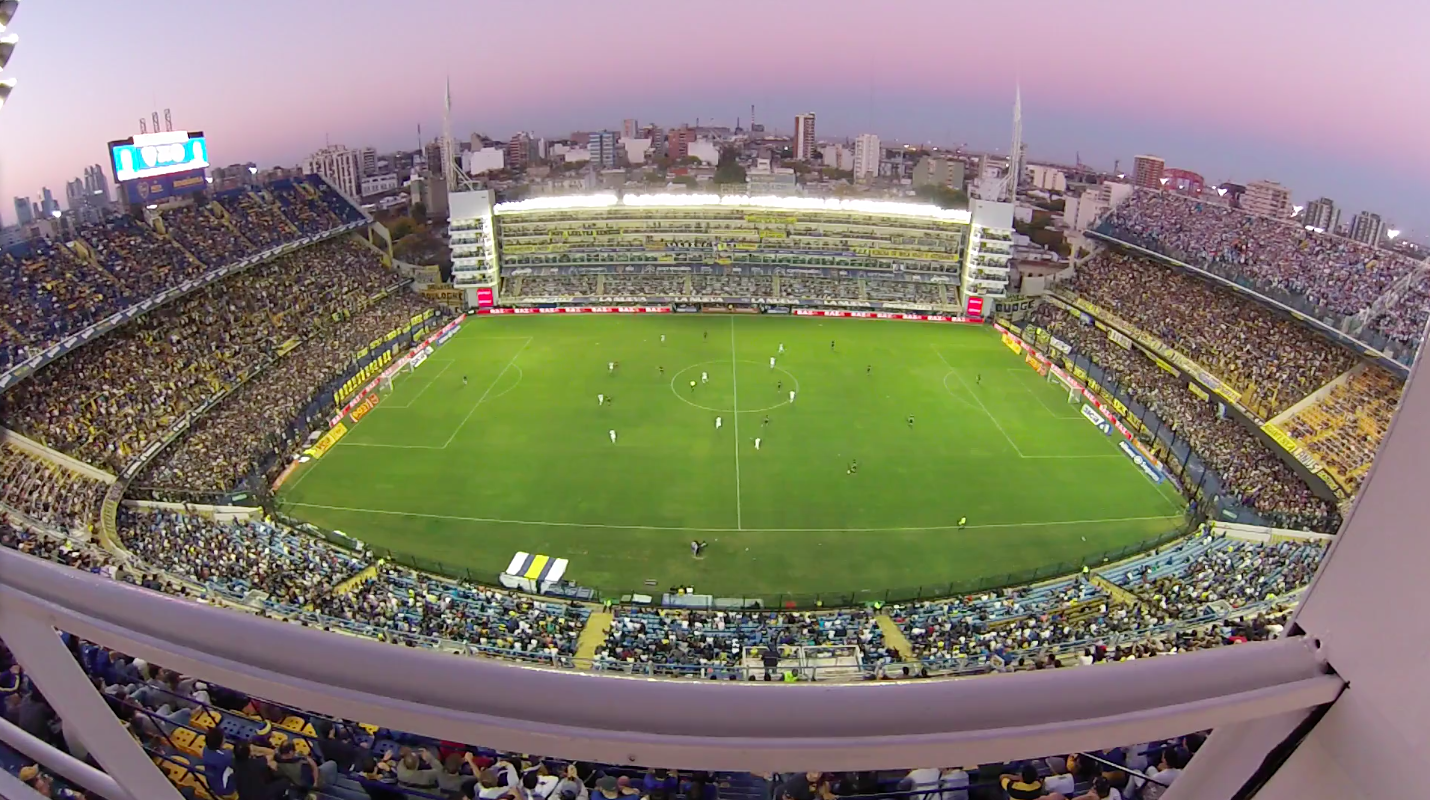
\includegraphics[width=\linewidth]{./images/Crop_Antes.png}
      \caption{Un cuadro del video de un partido entre Boca e Independiente.
      \label{fig:crop-antes}}
    \end{minipage}
    \begin{minipage}[t]{.45\textwidth}
      \centering
      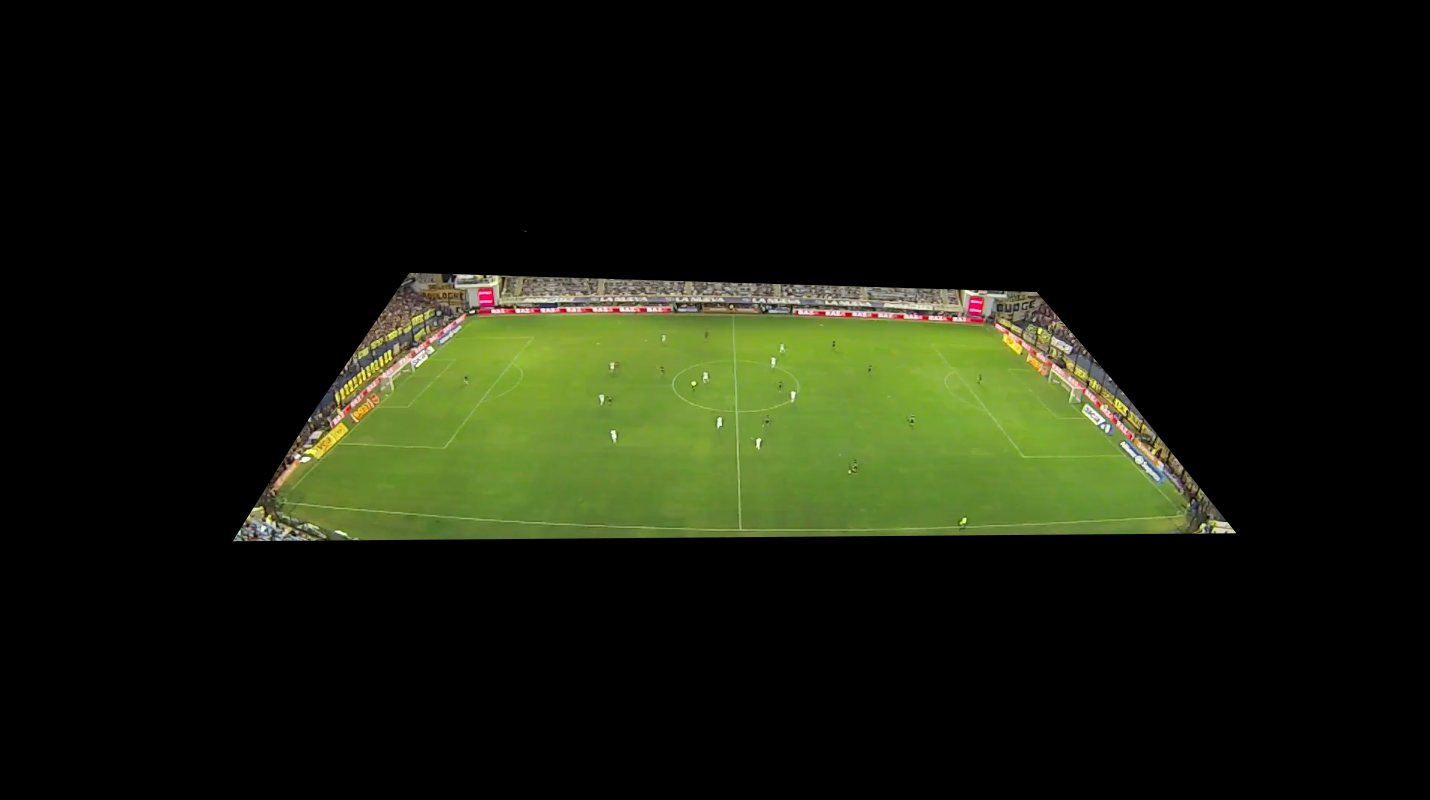
\includegraphics[width=\linewidth]{./images/Crop_Despues.png}
      \caption{El mismo cuadro, luego de aplicarle la operación \textit{Crop}.
      \label{fig:crop-despues}}
    \end{minipage}
\end{figure}

\subsection{Substracción de Fondo por Valor de Energía}

Se implementó el método de eliminación de fondo descripto en
\cite{papers-tanos}, para eliminación de sectores que corresponden al
verde del césped de la cancha o líneas pintadas sobre el mismo basado en una
medición de la variación del color de cada píxel (energía).

Este no resultó ser un método apropiado debido a que el sistema de codificación
del video generaba muchos falsos negativos, sobre todo \textit{glitches}
alrededor de las líneas de la cancha, lo que les otorgaba a estos puntos un
mayor valor de energía del que realmente tendrían.

\subsection{Eliminación de Líneas}

Basado en la detección de líneas de Hough, se desarrolló un método similar que
detecta los tramos pintados de blanco en el césped de la cancha. El mismo
funciona aplicando un detector de bordes (se probaron resultados utilizando
tanto el método de Roberts como el de Canny), umbralizando el resultado, y
haciendo un análisis morfológico de las componentes conexas obtenidas luego de
la umbralización.

Respecto a la detección de líneas de Hough, este método es preferible debido
a que detecta todo tipo de forma que sea demasiado larga o ancha como para
ser un jugador (por ejemplo, el círculo central y medios círculos en las
áreas alrededor de los arcos).

\subsection{Eliminación del césped}

% TODO: Champo review esto
Para la eliminación del césped del campo de juego se requiere caracterizarlo
de alguna forma. Para esto, se realiza un simple muestreo de los colores de
la imagen recortada, es decir la imagen resultante luego aplicar la técnica
de \textit{crop}, detallada en \ref{subsec:crop-tribunas}. A partir de este
muestreo, se construye un histograma de colores y se determina como color del
césped al color con mayor frecuencia. En realidad, debido a pequeñas
fluctuaciones por cambios de iluminación y resolución, se toman un rango de
valores alrededor del color con mayor frecuencia.

\section{Contornos activos}
\label{sec:ac-extension}

Como se explica en Sección \ref{sec:ac-problemas}, cuando los objetos de
interés son complejos, la utilización del color promedio como única
característica distintiva no alcanza. Es por esto que varias de las mejoras
planteadas al algoritmo de Contornos Activos giran en torno a la selección de
características para representar a los objetos de interés. Esta Sección
describe cambios que se han incorporado para hacer el algoritmo más efectivo
ante un video correspondiente a un partido de fútbol.

Si bien el color promedio resulta insuficiente para caracterizar correctamente
al objeto, puede utilizarse en complemento con otras características. La más
intuitiva es la utilización de la varianza de color en el objeto de interés.

Además de estos indicadores estadísticos, se pueden utilizar varias valores
para caracterizar el objeto, en lugar de utilizar un solo valor como puede ser
el color promedio o la varianza. Para esto, por ejemplo, puede realizarse un
histograma de colores y seleccionar los picos más altos del histograma como
colores representativos del objeto.

\subsection{Características}

Se estudiaron varias posibilidades para la selección de características que
determinaran los contornos de los jugadores respecto al color de fondo.
Finalmente, se optó por utilizar tres características, correspondientes a los
valores de RGB de cada píxel. A continuación se detallan alternativas:
\begin{itemize}
  \item \textbf{Valores HSL}: Se tomaron, en vez de los valores de rojo, verde
    y azul, los valores de \textit{hue}, \textit{saturation} y
    \textit{lightning}.

  \item \textbf{Desviación Estándar}: Se tomaron seis características para cada
    píxel: color (RGB o HSL) y desviación estándar de ese píxel respecto a los
    demás píxeles en una ventana de 5 píxeles alrededor del mismo.

\end{itemize}

\subsubsection{Selección de características}

Las características de un jugador son seleccionadas en base a los valores
encontrados inicialmente dentro de un cuadrado de un ancho y alto especificado
por el operador, que depende del video siendo analizado. Entre los píxeles
abarcados por el área de ese cuadrado, se realiza un histograma en tres
dimensiones (cada dimensión corresponde a los valores de rojo, verde, y azul
respectivamente). Se toma el valor máximo de ese histograma como el color
principal, y las características para este jugador son tomadas de este valor.

\subsubsection{Aprendizaje de valores}

Se realiza un aprendizaje simple para cada característica

\subsection{Descriptores}
% TODO: Champo me cansé de escuchar que es esto y no tengo idea de a que se refiere
